\documentclass{standalone}
\usepackage{tikz}
\usetikzlibrary{patterns, positioning}
\usepackage[sfdefault]{ClearSans} %% option 'sfdefault' activates Clear Sans as the default text font
\usepackage[T1]{fontenc}

\begin{document}
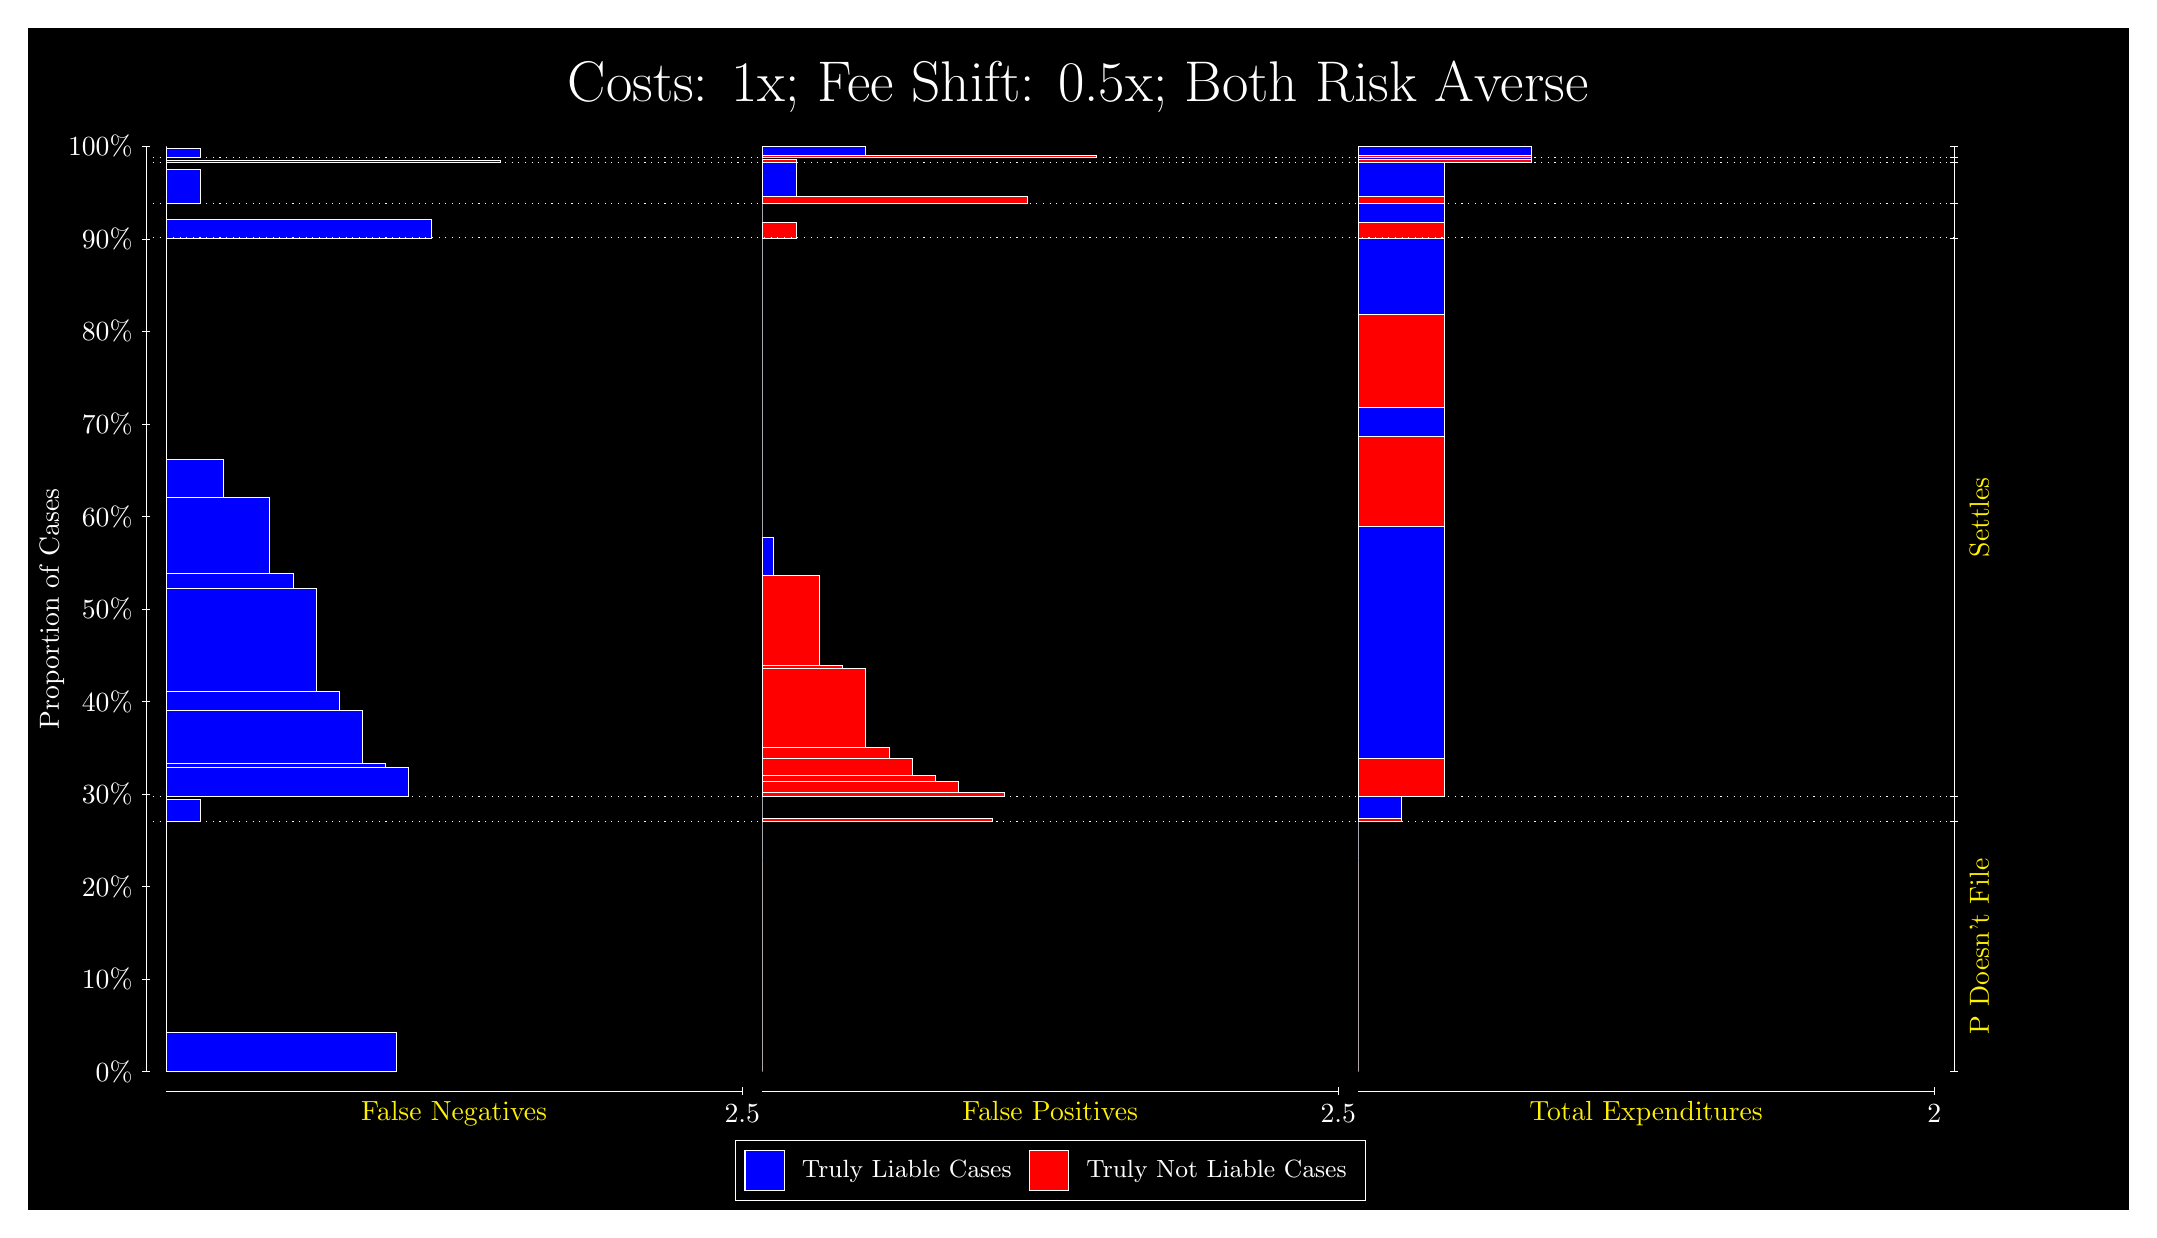
\begin{tikzpicture}
\draw[fill=black] (0,0) rectangle (26.667,15);
\draw[text=white] (0,13.5) rectangle (26.667,15) node[midway] {\huge Costs: 1x; Fee Shift: 0.5x; Both Risk Averse};
\draw[white, very thin] (1.5,1.75) -- (1.5,13.5);
\node[rotate=90, text=white, anchor=center] at (0.3, 7.625) {Proportion of Cases};
\draw[white, very thin] (1.45,1.75) -- (1.55,1.75);
\node[text=white, anchor=east] at (1.45, 1.75) {0\%};
\draw[white, very thin] (1.45,2.925) -- (1.55,2.925);
\node[text=white, anchor=east] at (1.45, 2.925) {10\%};
\draw[white, very thin] (1.45,4.1) -- (1.55,4.1);
\node[text=white, anchor=east] at (1.45, 4.1) {20\%};
\draw[white, very thin] (1.45,5.275) -- (1.55,5.275);
\node[text=white, anchor=east] at (1.45, 5.275) {30\%};
\draw[white, very thin] (1.45,6.45) -- (1.55,6.45);
\node[text=white, anchor=east] at (1.45, 6.45) {40\%};
\draw[white, very thin] (1.45,7.625) -- (1.55,7.625);
\node[text=white, anchor=east] at (1.45, 7.625) {50\%};
\draw[white, very thin] (1.45,8.8) -- (1.55,8.8);
\node[text=white, anchor=east] at (1.45, 8.8) {60\%};
\draw[white, very thin] (1.45,9.975) -- (1.55,9.975);
\node[text=white, anchor=east] at (1.45, 9.975) {70\%};
\draw[white, very thin] (1.45,11.15) -- (1.55,11.15);
\node[text=white, anchor=east] at (1.45, 11.15) {80\%};
\draw[white, very thin] (1.45,12.325) -- (1.55,12.325);
\node[text=white, anchor=east] at (1.45, 12.325) {90\%};
\draw[white, very thin] (1.45,13.5) -- (1.55,13.5);
\node[text=white, anchor=east] at (1.45, 13.5) {100\%};

\draw[white, very thin] (24.457,1.75) -- (24.457,13.5);
\draw[white, very thin] (24.407,1.75) -- (24.507,1.75);
\node[anchor=west] at (24.407, 1.75) {};
\draw[white, very thin] (24.407,4.9276) -- (24.507,4.9276);
\node[anchor=west] at (24.407, 4.9276) {};
\draw[white, very thin] (24.407,5.2399) -- (24.507,5.2399);
\node[anchor=west] at (24.407, 5.2399) {};
\draw[white, very thin] (24.407,12.338) -- (24.507,12.338);
\node[anchor=west] at (24.407, 12.338) {};
\draw[white, very thin] (24.407,12.776) -- (24.507,12.776);
\node[anchor=west] at (24.407, 12.776) {};
\draw[white, very thin] (24.407,13.3) -- (24.507,13.3);
\node[anchor=west] at (24.407, 13.3) {};
\draw[white, very thin] (24.407,13.361) -- (24.507,13.361);
\node[anchor=west] at (24.407, 13.361) {};
\draw[white, very thin] (24.407,13.5) -- (24.507,13.5);
\node[anchor=west] at (24.407, 13.5) {};

\draw[white, very thin, fill=blue] (1.75,1.75) rectangle (4.6775,2.248);
\draw[white, very thin, fill=red] (1.75,2.248) rectangle (1.75,4.9276);
\draw[white, very thin, fill=blue] (1.75,4.9276) rectangle (2.1891,5.2071);
\draw[white, very thin, fill=red] (1.75,5.2071) rectangle (1.75,5.2399);
\draw[white, very thin, fill=blue] (1.75,5.2399) rectangle (4.8239,5.6096);
\draw[white, very thin, fill=blue] (1.75,5.6096) rectangle (4.5312,5.6622);
\draw[white, very thin, fill=blue] (1.75,5.6622) rectangle (4.2384,6.332);
\draw[white, very thin, fill=blue] (1.75,6.332) rectangle (3.9457,6.5823);
\draw[white, very thin, fill=blue] (1.75,6.5823) rectangle (3.6529,7.8899);
\draw[white, very thin, fill=blue] (1.75,7.8899) rectangle (3.3602,8.0831);
\draw[white, very thin, fill=blue] (1.75,8.0831) rectangle (3.0674,9.047);
\draw[white, very thin, fill=blue] (1.75,9.047) rectangle (2.4819,9.5313);
\draw[white, very thin, fill=red] (1.75,9.5313) rectangle (1.75,12.338);
\draw[white, very thin, fill=blue] (1.75,12.338) rectangle (5.1167,12.575);
\draw[white, very thin, fill=red] (1.75,12.575) rectangle (1.75,12.776);
\draw[white, very thin, fill=blue] (1.75,12.776) rectangle (2.1891,13.206);
\draw[white, very thin, fill=red] (1.75,13.206) rectangle (1.75,13.3);
\draw[white, very thin, fill=blue] (1.75,13.3) rectangle (5.9949,13.329);
\draw[white, very thin, fill=red] (1.75,13.329) rectangle (1.75,13.361);
\draw[white, very thin, fill=blue] (1.75,13.361) rectangle (2.1891,13.471);
\draw[white, very thin, fill=red] (1.75,13.471) rectangle (1.75,13.5);
\draw[white, very thin, fill=red] (9.3189,1.75) rectangle (9.3189,4.4296);
\draw[white, very thin, fill=blue] (9.3189,4.4296) rectangle (9.3189,4.9276);
\draw[white, very thin, fill=red] (9.3189,4.9276) rectangle (12.246,4.9605);
\draw[white, very thin, fill=blue] (9.3189,4.9605) rectangle (9.3189,5.2399);
\draw[white, very thin, fill=red] (9.3189,5.2399) rectangle (12.393,5.3002);
\draw[white, very thin, fill=red] (9.3189,5.3002) rectangle (11.807,5.4392);
\draw[white, very thin, fill=red] (9.3189,5.4392) rectangle (11.515,5.5082);
\draw[white, very thin, fill=red] (9.3189,5.5082) rectangle (11.222,5.7305);
\draw[white, very thin, fill=red] (9.3189,5.7305) rectangle (10.929,5.8647);
\draw[white, very thin, fill=red] (9.3189,5.8647) rectangle (10.636,6.8658);
\draw[white, very thin, fill=red] (9.3189,6.8658) rectangle (10.344,6.9145);
\draw[white, very thin, fill=red] (9.3189,6.9145) rectangle (10.051,8.0465);
\draw[white, very thin, fill=blue] (9.3189,8.0465) rectangle (9.4652,8.5308);
\draw[white, very thin, fill=blue] (9.3189,8.5308) rectangle (9.3189,12.338);
\draw[white, very thin, fill=red] (9.3189,12.338) rectangle (9.758,12.538);
\draw[white, very thin, fill=blue] (9.3189,12.538) rectangle (9.3189,12.776);
\draw[white, very thin, fill=red] (9.3189,12.776) rectangle (12.686,12.87);
\draw[white, very thin, fill=blue] (9.3189,12.87) rectangle (9.758,13.3);
\draw[white, very thin, fill=red] (9.3189,13.3) rectangle (9.758,13.333);
\draw[white, very thin, fill=blue] (9.3189,13.333) rectangle (9.3189,13.361);
\draw[white, very thin, fill=red] (9.3189,13.361) rectangle (13.564,13.39);
\draw[white, very thin, fill=blue] (9.3189,13.39) rectangle (10.636,13.5);
\draw[white, very thin, fill=red] (16.888,1.75) rectangle (16.888,4.4296);
\draw[white, very thin, fill=blue] (16.888,4.4296) rectangle (16.888,4.9276);
\draw[white, very thin, fill=red] (16.888,4.9276) rectangle (17.437,4.9605);
\draw[white, very thin, fill=blue] (16.888,4.9605) rectangle (17.437,5.2399);
\draw[white, very thin, fill=red] (16.888,5.2399) rectangle (17.986,5.7305);
\draw[white, very thin, fill=blue] (16.888,5.7305) rectangle (17.986,8.6795);
\draw[white, very thin, fill=red] (16.888,8.6795) rectangle (17.986,9.8116);
\draw[white, very thin, fill=blue] (16.888,9.8116) rectangle (17.986,10.181);
\draw[white, very thin, fill=red] (16.888,10.181) rectangle (17.986,11.365);
\draw[white, very thin, fill=blue] (16.888,11.365) rectangle (17.986,12.338);
\draw[white, very thin, fill=red] (16.888,12.338) rectangle (17.986,12.538);
\draw[white, very thin, fill=blue] (16.888,12.538) rectangle (17.986,12.776);
\draw[white, very thin, fill=red] (16.888,12.776) rectangle (17.986,12.87);
\draw[white, very thin, fill=blue] (16.888,12.87) rectangle (17.986,13.3);
\draw[white, very thin, fill=red] (16.888,13.3) rectangle (19.083,13.333);
\draw[white, very thin, fill=blue] (16.888,13.333) rectangle (19.083,13.361);
\draw[white, very thin, fill=red] (16.888,13.361) rectangle (19.083,13.39);
\draw[white, very thin, fill=blue] (16.888,13.39) rectangle (19.083,13.5);
\draw[white, dotted] (1.5,4.9276) -- (24.457,4.9276);
\draw[white, dotted] (1.5,5.2399) -- (24.457,5.2399);
\draw[white, dotted] (1.5,12.338) -- (24.457,12.338);
\draw[white, dotted] (1.5,12.776) -- (24.457,12.776);
\draw[white, dotted] (1.5,13.3) -- (24.457,13.3);
\draw[white, dotted] (1.5,13.361) -- (24.457,13.361);
\draw[white, very thin] (1.75,1.5) -- (9.0689,1.5);
\node[text=yellow, anchor=north] at (5.4094, 1.5) {False Negatives};
\draw[white, very thin] (9.0689,1.45) -- (9.0689,1.55);
\node[text=white, anchor=north] at (9.0689, 1.45) {2.5};

\draw[white, very thin] (9.3189,1.5) -- (16.638,1.5);
\node[text=yellow, anchor=north] at (12.978, 1.5) {False Positives};
\draw[white, very thin] (16.638,1.45) -- (16.638,1.55);
\node[text=white, anchor=north] at (16.638, 1.45) {2.5};

\draw[white, very thin] (16.888,1.5) -- (24.207,1.5);
\node[text=yellow, anchor=north] at (20.547, 1.5) {Total Expenditures};
\draw[white, very thin] (24.207,1.45) -- (24.207,1.55);
\node[text=white, anchor=north] at (24.207, 1.45) {2};

\node[text=yellow, centered, rotate=90] at (24.777, 3.3388) {P Doesn't File};

\node[text=yellow, centered, rotate=90] at (24.777, 8.7889) {Settles};





\draw (12.978300999999998,1.5) node[draw=none] (baseCoordinate) {};
\begin{scope}[align=center]
        \matrix[scale=0.5, draw=white, below=0.5cm of baseCoordinate, nodes={draw}, column sep=0.1cm]{
            \node[rectangle, draw, minimum width=0.5cm, minimum height=0.5cm, fill=blue] {}; &
            \node[draw=none, font=\small, text=white] (B) {Truly Liable Cases}; &
            \node[rectangle, draw, minimum width=0.5cm, minimum height=0.5cm, fill=red] {}; &
            \node[draw=none, font=\small, text=white] (B) {Truly Not Liable Cases}; \\
            };
\end{scope}

\end{tikzpicture}
\end{document}